%\PassOptionsToPackage{draft}{graphicx}
\documentclass[aspectratio=149, structureblod, xcolor=table]{beamer}
\usetheme{Warsaw}
%\useoutertheme{split}
\usefonttheme[onlymath]{serif}

\usepackage[utf8]{inputenc}
\usepackage[spanish]{babel}
\spanishdecimal{.}

%\usepackage{geometry}
%\geometry{right=0cm, left=0cm}
\usepackage{anyfontsize}
\usepackage{ragged2e}
\usepackage{graphicx}
\usepackage{enumitem}
%\usepackage{subfigure}
\usepackage{subcaption}
%\usepackage[absolute,overlay]{textpos}		% textblock
\usepackage[export]{adjustbox}
%\usepackage{float}
\usepackage{floatrow}
\usepackage{caption}
\usepackage{amsmath}
\usepackage{tikz}
\usetikzlibrary{arrows.meta}
\usepackage{etoolbox}
\usepackage{calc}
\usepackage{setspace}
\usepackage{xcolor}
\usepackage{array}
\usepackage{background}
\backgroundsetup{
    placement=center,
    position={0.0758,-0.0496},
    scale=120,
    angle=0,
    contents={
\includegraphics{Migala_logo_5_2.pdf}},
    opacity=0.07
}
\setbeamertemplate{background}{\BgMaterial}

\newcommand\Wider[2][3em]{
	\makebox[\linewidth][c]{
		\begin{minipage}{\dimexpr\textwidth+#1\relax}
			\raggedright#2
		\end{minipage}
	}
}

\makeatletter
\newcommand{\noheadline}{
	\setbeamertemplate{headline}[default]
	\def\beamer@entrycode{\vspace{-2.147ex}}
	\backgroundsetup{position={0.0758,-0.046225}}
}
\makeatother


\usepackage{printlen}
\uselengthunit{in}

\beamertemplatenavigationsymbolsempty

\definecolor{rosaOscuro}{RGB}{88,19,62}
\definecolor{rosaMedio}{RGB}{136,30,111}
\definecolor{rosaClaro}{RGB}{255,245,255}
\definecolor{rosaClaroDos}{RGB}{171,37,122}
\definecolor{rosaBarras}{RGB}{190,41,138}

\setbeamercolor{palette primary}{fg=white, bg=rosaOscuro}
\setbeamercolor{palette secondary}{fg=green, bg=yellow}
\setbeamercolor{palette tertiary}{fg=green, bg=yellow}
\setbeamercolor{palette quaternary}{fg=white, bg=rosaMedio}

\setbeamercolor{item}{fg=rosaMedio}
\setbeamercolor{section in toc}{fg=rosaOscuro}

\setbeamerfont{block title}{shape=\it}
\addtobeamertemplate{block begin}{}{\justifying\indent}

%\setbeamercolor{block title}{fg=white, bg=verdeMedio}
\setbeamercolor{block body}{fg=black, bg=white}
%\setbeamercolor{block title alerted}{fg=white, bg=pink}
%\setbeamercolor{block body alerted}{fg=black, bg=white}
%\setbeamercolor{block title example}{fg=white, bg=pink}
%\setbeamercolor{block body example}{fg=pink, bg=white}

\setbeamercolor{normal text}{fg=black, bg=rosaClaro}
%\setbeamercolor{section in head/foot}{bg=rosaOscuro}
%\setbeamercolor{subsection in head/foot}{bg=rosaMedio}

\makeatletter
\setbeamercolor{item projected}{bg=rosaMedio}
\setlist[itemize]{itemsep=10pt, label=\raise0.2pt\beamer@usesphere{item projected}{bigsphere}}
\makeatother

\setbeamertemplate{headline}{
  \leavevmode%
  \begin{beamercolorbox}[wd=.5\paperwidth,ht=2.5ex,dp=1.125ex,leftskip=.3cm plus1fill, shadow=true, rightskip=.3cm]{section in head/foot}%
    \usebeamertemplate{section in head/foot}
    %\usebeamerfont{section in head/foot}\insertsection%
  \end{beamercolorbox}%
  \begin{beamercolorbox}[wd=.5\paperwidth,ht=2.5ex,dp=1.125ex,shadow=true,leftskip=.3cm,rightskip=.3cm plus1fil]{subsection in head/foot}%
  	\usebeamertemplate{subsection in head/foot}
  	%\usebeamerfont{subsection in head/foot}\insertsubsection%%
  \end{beamercolorbox}%
  \vskip1.9pt%
}

%\setbeamercolor{author in head/foot}{bg=rosaMedio}
%\setbeamercolor{title in head/foot}{bg=rosaOscuro}
\newcommand{\numdiap}{\insertframenumber /\inserttotalframenumber}
\setbeamertemplate{footline}{
	\leavevmode%
	%\hbox{
		\begin{beamercolorbox}[wd=.5\paperwidth,ht=2.5ex,dp=1.125ex,leftskip=.3cm plus1fill,rightskip=.3cm]{author in head/foot}%
			\usebeamerfont{author in head/foot}\insertshortauthor
		\end{beamercolorbox}%
		\begin{beamercolorbox}[wd=.5\paperwidth,ht=2.5ex,dp=1.125ex,leftskip=.3cm,rightskip=.3cm plus1fil]{title in head/foot}%
			\usebeamerfont{title in head/foot}\insertshorttitle \hfill \numdiap
		\end{beamercolorbox}
	%}%
	\vskip0pt%
}

\setbeamertemplate{title page}{
	\begin{center}%
		%\begin{minipage}{4cm}
		\begin{beamercolorbox}[sep=15pt, center]{}
			\inserttitlegraphic \hspace{0.6cm} \raisebox{10pt}{\centering \scshape \LARGE \insertinstitute}
		\end{beamercolorbox}%\vfill%
		\begin{beamercolorbox}[sep=18pt, center, shadow=true, rounded=true]{title}
			\Large \textit{\inserttitle}
		\end{beamercolorbox}%\vskip 7pt%
		\begin{beamercolorbox}[sep=18pt, center, shadow=true, rounded=true]{author}
			\centering
			\insertauthor
		\end{beamercolorbox}\vfill%
		\begin{beamercolorbox}[sep=8pt, center, shadow=true, rounded=true]{date}
			\insertdate
		\end{beamercolorbox}%
		%\end{minipage}
	\end{center}
}

%\makeatletter
	\newcount\c@p
	\newcount\c@m
	\newcount\c@pp
	\newcount\c@mm
	\def\insertsectionnavigation#1{%
		\hbox to #1{%
			\vbox{{
				\usebeamerfont{section in head/foot}\usebeamercolor[fg]{section in head/foot}%
				\vskip0.5625ex%
				\def\slideentry##1##2##3##4##5##6{}%
				\def\sectionentry##1##2##3##4##5{%
					\ifnum##5=\c@part%
						\def\insertsectionhead{##2}%
						\def\insertsectionheadnumber{##1}%
						\def\insertpartheadnumber{##5}%
						\c@p=\c@section%
						\c@m=\c@section%
						\c@pp=\c@section%
						\c@mm=\c@section%
						\advance\c@m by -1 %
				 		\advance\c@p by 1 %
						\advance\c@mm by -2 %
						\advance\c@pp by 2 %
						%
						\ifnum \c@section=1
							\ifnum\c@section=##1%
								\setbox\beamer@tempbox=\hbox{%
									\hyperlink{Navigation##3}{\hbox to #1{%
										{\hskip0.3cm\usebeamertemplate{section in head/foot}\hskip0.3cm}}}}%
							\else%
								\ifnum##1=\c@p%
									\setbox\beamer@tempbox=\hbox{%
										\hyperlink{Navigation##3}{\hbox to #1{%
											{\hskip0.3cm\usebeamertemplate{section in head/foot shaded}\hskip0.3cm}}}}%
								\else%
									\ifnum##1=\c@pp%
										\setbox\beamer@tempbox=\hbox{%
											\hyperlink{Navigation##3}{\hbox to #1{%
												{\hskip0.3cm\usebeamertemplate{section in head/foot shaded}\hskip0.3cm}}}}
									\else%
									\fi%
								\fi%
							\fi%% 
						\else%
							\ifnum \c@section=\beamer@sectionmax
								\ifnum\c@section=##1%
									\setbox\beamer@tempbox=\hbox{%
				 						\hyperlink{Navigation##3}{\hbox to #1{%
					 						{\hskip0.3cm\usebeamertemplate{section in head/foot}\hskip0.3cm}}}}%
								\else%
									\ifnum##1=\c@m%
										\setbox\beamer@tempbox=\hbox{%
					 						\hyperlink{Navigation##3}{\hbox to #1{%
												{\hskip0.3cm\usebeamertemplate{section in head/foot shaded}\hskip0.3cm}}}}
					 				\else%
										\ifnum##1=\c@mm%
											\setbox\beamer@tempbox=\hbox{%
												\hyperlink{Navigation##3}{\hbox to #1{%
													{\hskip0.3cm\usebeamertemplate{section in head/foot shaded}\hskip0.3cm
													}}}}%
										\else%
										\fi%
									\fi%
								\fi%%
							\else%
								\ifnum\c@section=##1%
									\setbox\beamer@tempbox=\hbox{%
										\hyperlink{Navigation##3}{\hbox to #1{%
											{\hskip0.3cm\usebeamertemplate{section in head/foot}\hskip0.3cm}}}}%
								\else%
									\ifnum##1=\c@m%
										\setbox\beamer@tempbox=\hbox{%
											\hyperlink{Navigation##3}{\hbox to #1{%
												{\hskip0.3cm\usebeamertemplate{section in head/foot shaded}\hskip0.3cm}}}}
									\else%
										\ifnum##1=\c@p%
											\setbox\beamer@tempbox=\hbox{%
												\hyperlink{Navigation##3}{\hbox to #1{%
													{\hskip0.3cm\usebeamertemplate{section in head/foot shaded}\hskip0.3cm
													}}}}%
					 					\else%
										\fi%
									\fi%
					 			\fi%
							\fi%
						\fi%
						\ht\beamer@tempbox=1.6875ex%
						\dp\beamer@tempbox=0.75ex%
						\box\beamer@tempbox
					\fi
				}%
				\dohead\vskip0.5625ex
			}}\hfil
		}
	}

	\setbeamertemplate{headline}{
		\leavevmode%
		\@tempdimb=3em%
		\ifdim\@tempdimb>0pt%
			\advance\@tempdimb by 1.825ex%
			\begin{beamercolorbox}[wd=.5\paperwidth,ht=\@tempdimb]{section in head/foot}%
				\vbox to\@tempdimb{\vfil\insertsectionnavigation{.5\paperwidth}\vfil}%
			\end{beamercolorbox}%
			\begin{beamercolorbox}[wd=.5\paperwidth,ht=\@tempdimb]{subsection in head/foot}%
				\vbox to\@tempdimb{\vfil\insertsubsectionnavigation{.5\paperwidth}\vfil}%
			\end{beamercolorbox}%
		\fi%
	}
\makeatother

\setbeamertemplate{caption}[numbered]

\setbeamerfont{subsection in toc}{size=\scriptsize}

\setbeamertemplate{bibliography item}{\insertbiblabel}
\setbeamercolor{bibliography item}{fg=rosaOscuro}
\setbeamercolor{bibliography entry author}{fg=rosaOscuro}
\setbeamercolor{bibliography entry location}{fg=rosaClaroDos}
\setbeamercolor{bibliography entry note}{fg=rosaClaroDos}
	
\title[Encuesta Partido Migala]{Análisis de datos de encuesta a potenciales miembros del Partido Migala}
%\subtitle{Subtítulo}
\author[J. Alberto López L.]{José Alberto López López}
\institute{Partido Migala}
\date{\today}
\titlegraphic{
\includegraphics[width=1.3cm]{Migala_logo_5}}

\let\oldtableofcontents\tableofcontents
\def\tableofcontents{\setlength{\parskip}{1ex}\oldtableofcontents}

%\setbeamerfont{frame text}{size=\Huge}
%\includeonlyframes{current}



\begin{document}


\justifying
\small
\frame[plain]{\titlepage}


{
\noheadline
\begin{frame}{Contenido de la presentación}
\tableofcontents
\end{frame}
}


{
\noheadline
\begin{frame}{Notas preliminares}
\fontsize{10}{10}\selectfont
\begin{itemize}
\item La encuesta tuvo un total de 7501 participaciones.
\item Hubo un total de 1468 participantes (el 19.57\%) que, a lo mucho, solo respondieron las primeras dos preguntas (fecha de nacimiento y nacionalidad), saltándose todo lo demás y dejándolo vacío. Razón por la cuál en muchas de las gráficas se verá este número de nulos.
\item El tiempo promedio empleado para responder la encuesta de estos 1468 fue de 5min, mientras que el de los restantes fue de 27min.
\item Se reemplazaron 52 fechas de nacimiento que eran menores a 1920 por 1980.
\item Se reemplazaron 134 fechas de nacimiento que eran mayores a 2018 por 2010.
\item La marca \textit{r\,$>$1} en el título de una diapositiva significa que el encuestado podía seleccionar más de una respuesta a la pregunta en cuestión, por lo que el conteo de la gráfica puede ser más grande que el de participantes.
\end{itemize}
\end{frame}
}


\section{Datos generales de los encuestados}
\frame[noframenumbering, plain]{\tableofcontents[currentsection]}


\begin{frame}{Panorama de vacíos (hacer zoom)}
\vspace{-2.5pt}
\Wider[1.8cm]{\includegraphics{img/Vacios.pdf}}
\end{frame}

\begin{frame}{Edad}

El promedio de edad de los encuestados fue de 24.11 años.\vspace{0.3cm}

\Wider[1.3cm]{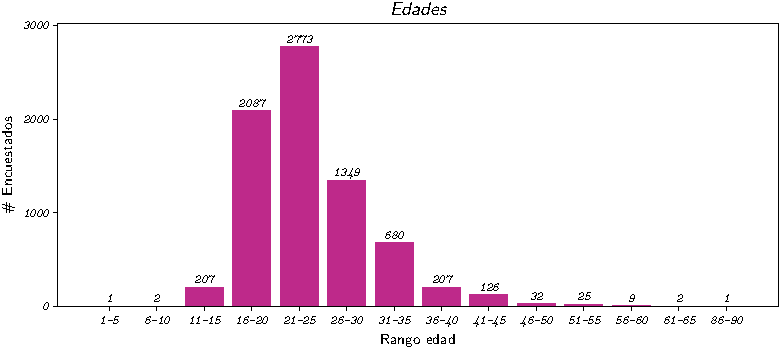
\includegraphics{img/Edades.pdf}}
\end{frame}

\begin{frame}{Nacionalidad}
\Wider[1.3cm]{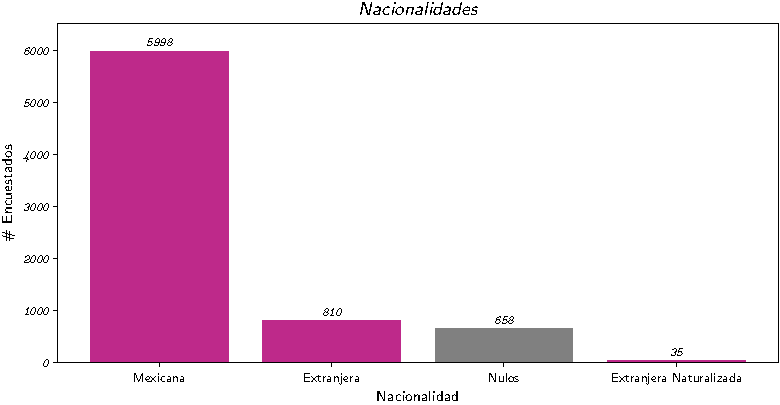
\includegraphics{img/Nacionalidad.pdf}}
\end{frame}

\begin{frame}{Género}
\Wider[1.3cm]{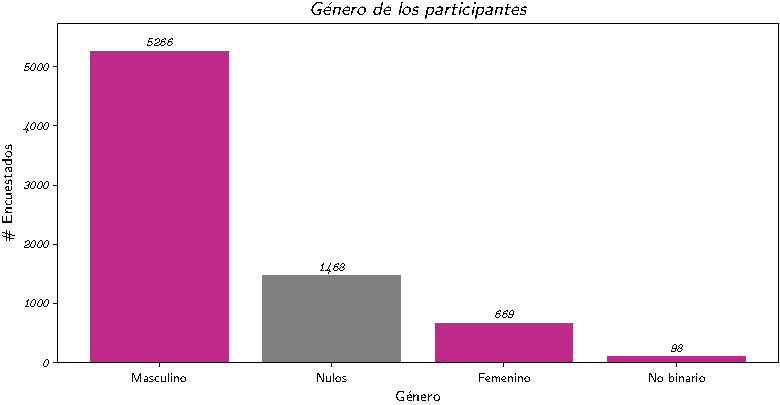
\includegraphics{img/Genero.pdf}}
\end{frame}

\begin{frame}{Discapacidad}
\Wider[1.3cm]{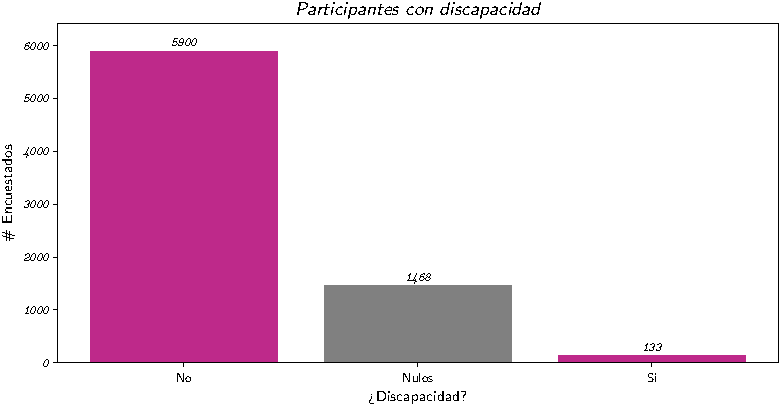
\includegraphics{img/Discapacidad.pdf}}
\end{frame}


\section{Ubicación geográfica}
\frame[noframenumbering, plain]{\tableofcontents[currentsection, subsectionstyle=shaded]}

\begin{frame}{Entidad de residencia}
\Wider[1.3cm]{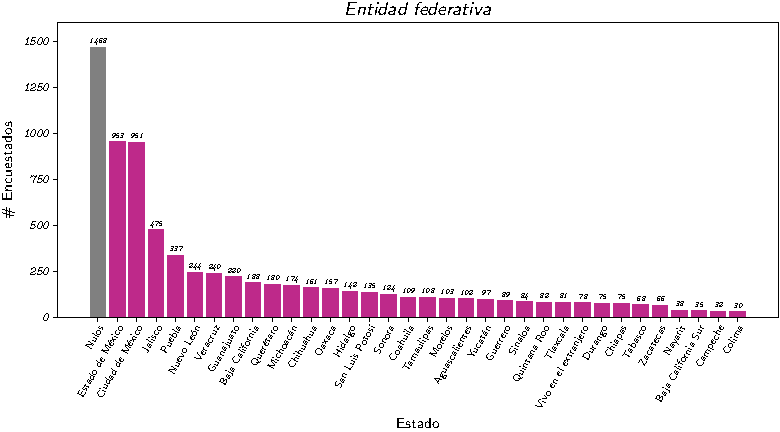
\includegraphics{img/Entidad_federativa.pdf}}
\end{frame}

\begin{frame}{Entidad de residencia}
\Wider[1.3cm]{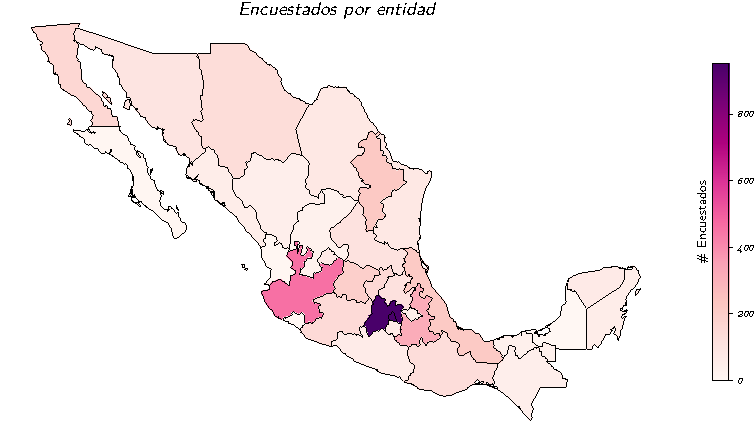
\includegraphics{img/Mapa_Mexico.pdf}}
\end{frame}

\subsection{Participación por estado}
\frame[noframenumbering, plain]{\tableofcontents[sectionstyle=shaded, currentsection, currentsubsection]}

\begin{frame}[noframenumbering, plain]
\setlength{\parskip}{8pt}
\textit{Nota:}

Por falta de tiempo, solo se realizó el conteo de participantes por estado para la CDMX.

Cualquier estado adicional que se requiera, sobre pedido.
\end{frame}

\begin{frame}{CDMX}
\Wider[1.3cm]{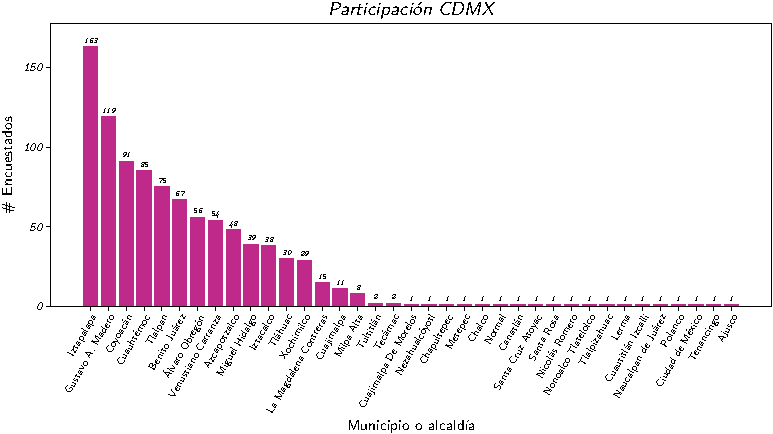
\includegraphics{img/Municipio.pdf}}
\end{frame}

\begin{frame}{CDMX}
\centering
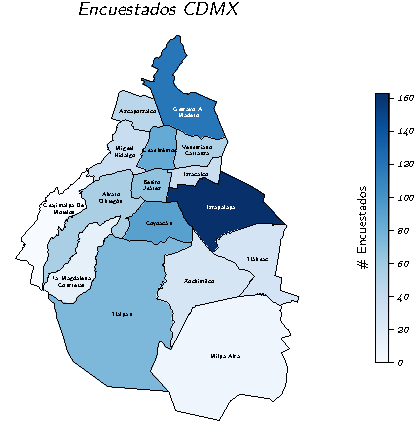
\includegraphics{img/Mapa_CDMX.pdf}
\end{frame}

\subsection{Viviendo en el extranjero}
\frame[noframenumbering, plain]{\tableofcontents[sectionstyle=shaded, currentsection, currentsubsection]}

\begin{frame}{Participantes en el extranjero}
\renewcommand{\arraystretch}{0.57}
\vspace{-9pt}
\rowcolors{2}{rosaMedio!30!white}{}
\begin{table}[H]
\begin{tabular}{>{\tiny} l >{\tiny} c >{\tiny} c}
\rowcolor{rosaMedio} \rule{0pt}{7pt} \textit{\fontsize{7.5}{7.5}\selectfont \color{white} País} & \textit{\fontsize{7.5}{7.5}\selectfont \color{white} \# Encuestados} & \textit{\fontsize{7.5}{7.5}\selectfont \color{white} Años viviendo (promedio)} \\[1pt]
E.U.A. & 34 & 4.29 \\
Alemania & 5 & 6 \\
Francia & 5 & 2 \\
España & 5 & 9 \\
Australia & 3 & 2 \\
Suecia & 2 & 3 \\
Perú & 2 & 20.5 \\
Canadá & 2 & 4 \\
Colombia & 2 & 21 \\
Argentina & 2 & 11 \\
Ecuador & 2 & 16 \\
Finlandia & 1 & 9 \\
Suiza & 1 & 5 \\
Portugal & 1 & 0 \\
Países Bajos & 1 & 2 \\
Italia & 1 & 1 \\
Costa Rica & 1 & 20 \\
Chile & 1 & 26 \\
Chequia & 1 & 1 \\
Bélgica & 1 & 13 \\
Brunei Darussalam & 1 & 1 \\
Brasil & 1 & 2 \\
Bolivia & 1 & 18 \\
Austria & 1 & 4 \\
Venezuela & 1 & 19
\end{tabular}
\end{table}

\end{frame}

\section{Ocupaciones y estudios}
\frame[noframenumbering, plain]{\tableofcontents[currentsection]}


\begin{frame}{Ocupación \hfill \textit{r\,$>$1}}
\Wider[1.3cm]{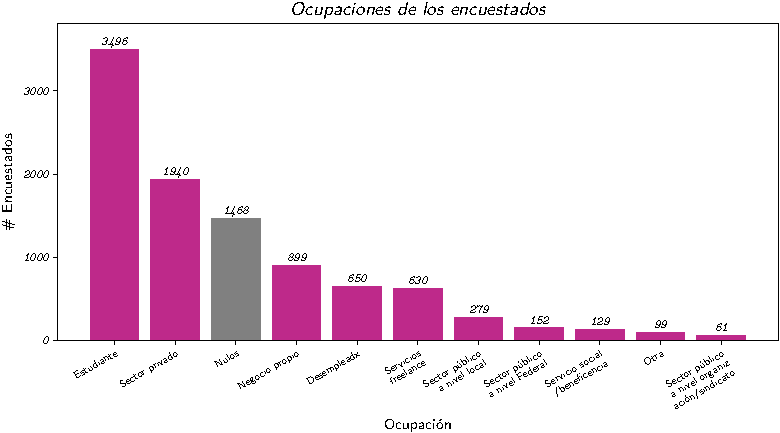
\includegraphics{img/Ocupacion.pdf}}
\end{frame}

\begin{frame}{Grado de estudios}
\Wider[1.3cm]{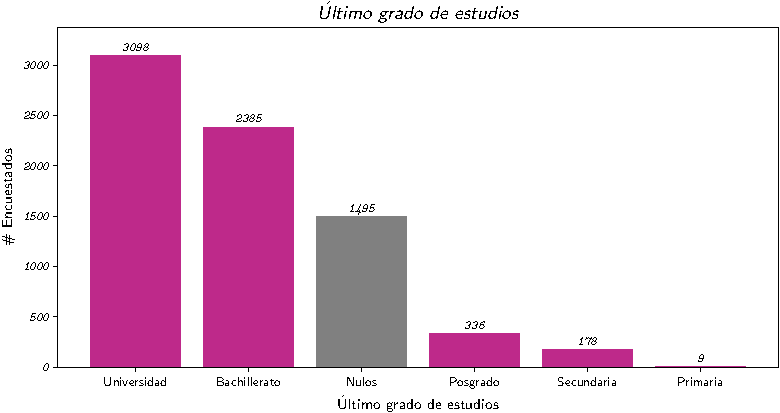
\includegraphics{img/Grado_estudios.pdf}}
\end{frame}

\begin{frame}{¿Trabajas en lo que estudiaste?}
\Wider[1.3cm]{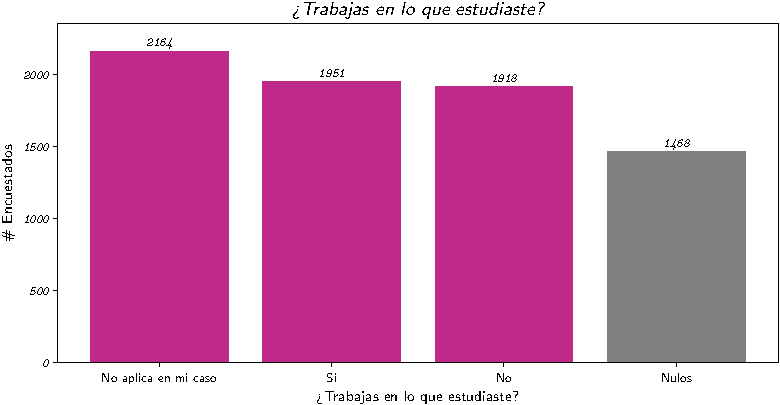
\includegraphics{img/Trabajas_en_lo_que_estudiaste.pdf}}
\end{frame}

\begin{frame}{Área de estudio \hfill \textit{r\,$>$1}}
\Wider[1.3cm]{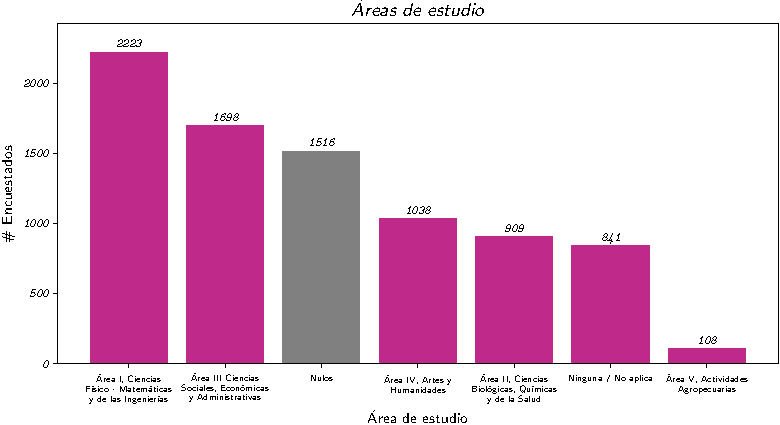
\includegraphics{img/Area_de_estudio.pdf}}
\end{frame}

\begin{frame}{Actividades extra \hfill \textit{r\,$>$1}}
Cabe destacar que en esta pregunta hubo mucha participación en el campo \textit{Actividad específica}, el cuál debía ser descrito manualmente por los usuarios.\vspace{0.2cm}

\Wider[1.3cm]{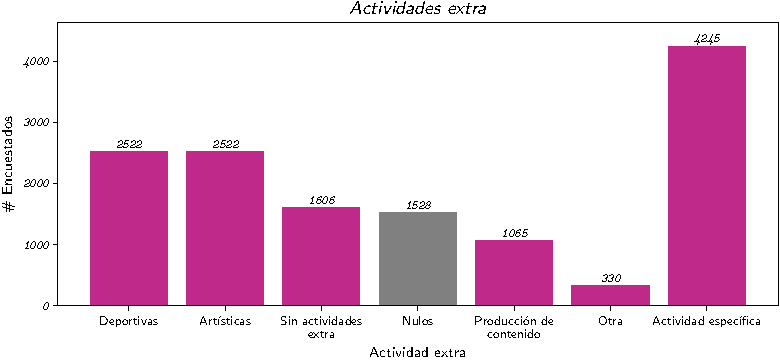
\includegraphics{img/Actividades_extra.pdf}}
\end{frame}

\begin{frame}{Actividades extra \hfill \textit{r\,$>$1}}
\Wider[1.3cm]{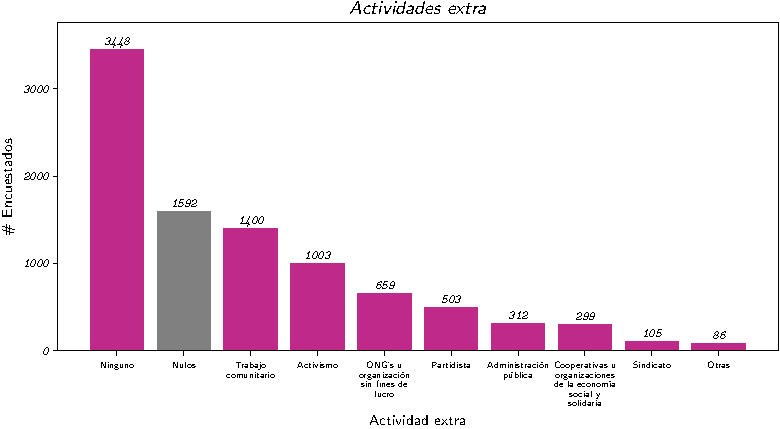
\includegraphics{img/Activismo.pdf}}
\end{frame}

\begin{frame}{Actividades políticas y/o sociales y conocimientos técnicos}
Los campos de: \textit{Actividades políticas y/o sociales} y de \textit{Conocimientos técnicos} debían ser llenados manualmente por los encuestados, especificando el tipo de actividad o conocimiento.
\vspace{10pt}
\begin{itemize}
\item En el campo \textit{Actividades políticas y/o sociales}, un total de 5181 encuestados se tomaron el tiempo para describir su actividad.
\item En el campo \textit{Conocimientos técnicos}, lo hicieron 5301 encuestados.
\end{itemize}
\end{frame}


\section{¿Cómo participarían?}
\frame[noframenumbering, plain]{\tableofcontents[currentsection]}


\begin{frame}{¿Cómo te gustaría participar en este proyecto?}
\Wider[1.3cm]{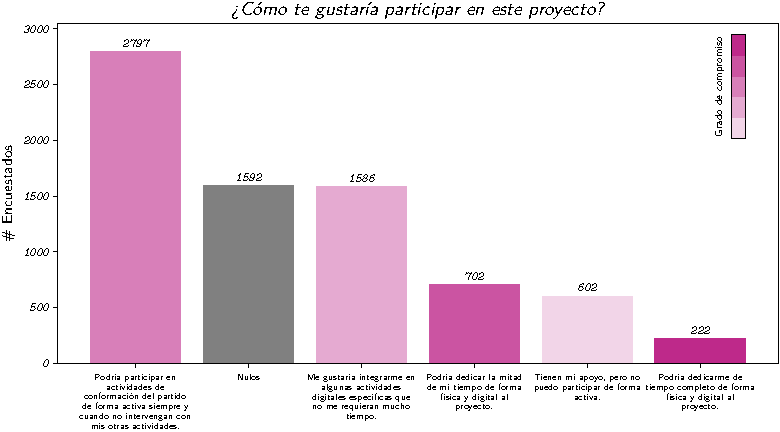
\includegraphics{img/Como_te_gustaria_participar.pdf}}
\end{frame}

\begin{frame}{Actividades para participar \hfill \textit{r\,$>$1}}
\Wider[1.3cm]{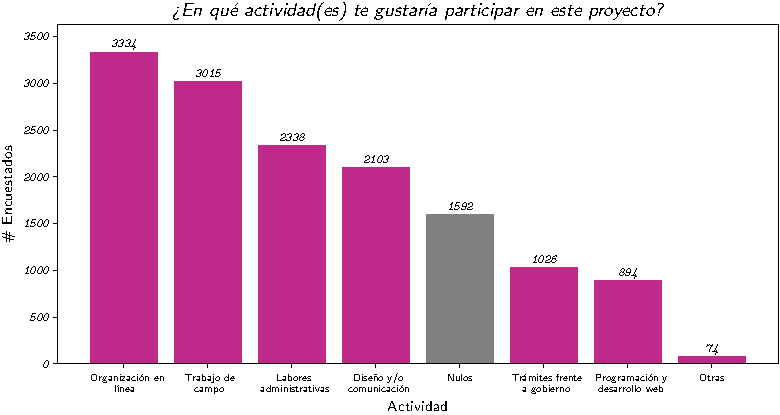
\includegraphics{img/En_que_actividades_te_gustaria_participar.pdf}}
\end{frame}

\begin{frame}{Disponibilidad}
\Wider[1.3cm]{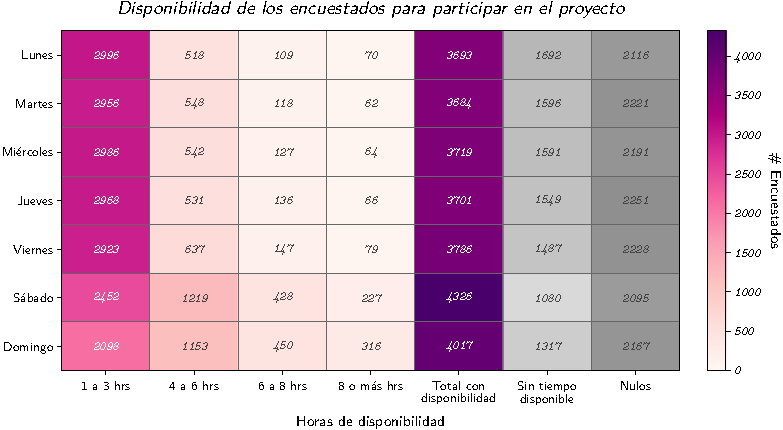
\includegraphics{img/Disponibilidad.pdf}}
\end{frame}

\begin{frame}{Disponibilidad (días por semana)}
\Wider[1.3cm]{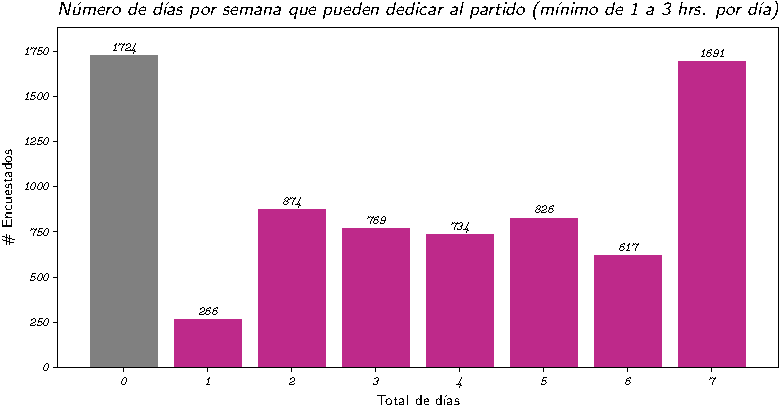
\includegraphics{img/Disponibilidad_dias.pdf}}
\end{frame}

\begin{frame}{Disponibilidad (horas por semana)}
\scriptsize
Suponiendo que los que seleccionaron de 1 a 3 hrs. trabajan un promedio de 2 hrs.; los de 4 a 6 hrs. un promedio de 5 hrs.; los de 6 a 8 hrs.: 7 hrs.; y los de 8 hrs. o más: 10 hrs.
La distribución de horas a la semana que pueden dedicar los participantes queda de la siguiente manera:\vspace{5pt}

\Wider[1.3cm]{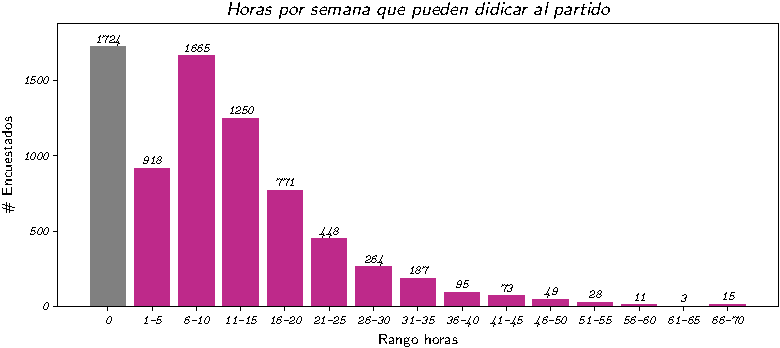
\includegraphics{img/Disponibilidad_horas.pdf}}
\end{frame}


\section{Conectividad y uso de redes sociales}
\frame[noframenumbering, plain]{\tableofcontents[currentsection]}


\begin{frame}{Conexión a Internet \hfill \textit{r\,$>$1}}
\Wider[1.3cm]{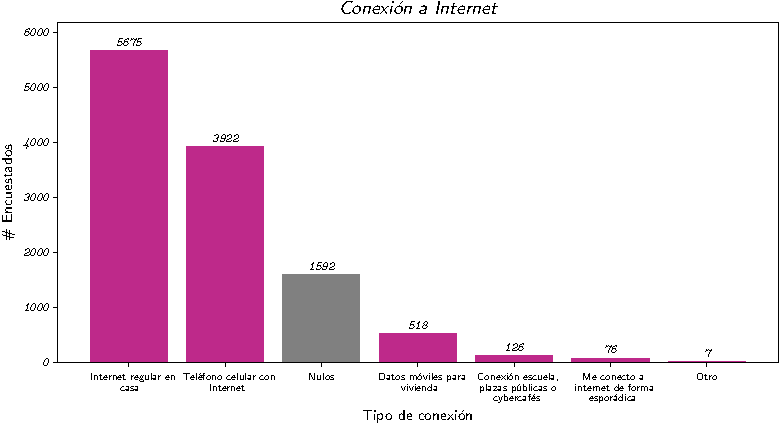
\includegraphics{img/Conexion_Internet.pdf}}
\end{frame}

\begin{frame}{Faimiliaridad con TI}
\Wider[1.3cm]{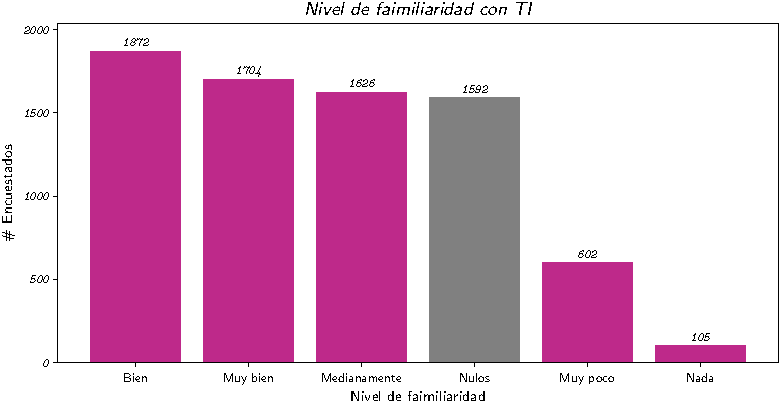
\includegraphics{img/Familiaridad_TI.pdf}}
\end{frame}

\begin{frame}{Uso de redes sociales \hfill \textit{r\,$>$1}}
\Wider[1.3cm]{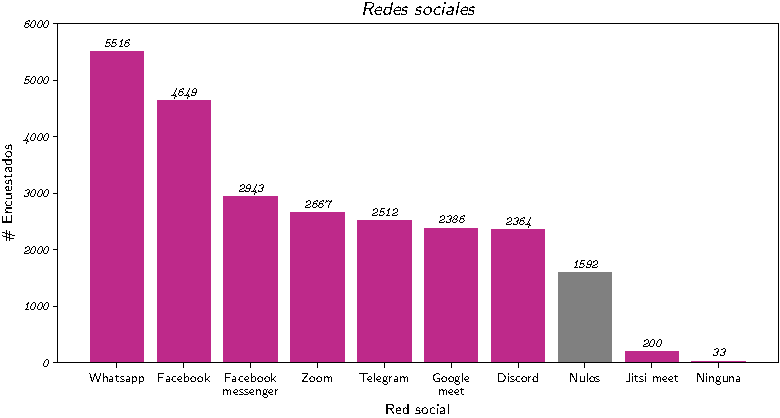
\includegraphics{img/Redes_sociales.pdf}}
\end{frame}

{
\noheadline
\begin{frame}{Notas finales}
\setlength{\parskip}{8pt}
\fontsize{10}{10}\selectfont
La información presentada corresponde en su mayoría a un análisis básico.
De requerirse, se pueden hacer un análisis más profundos, por ejemplo:
\begin{itemize}
\item Se puede extraer información de los campos que se llenaron manualmente, desde la lista completa de las descripciones hasta una búsqueda basada en patrones de palabras para filtrar información de interés.

\item Se pueden hacer consultas más complejas para obtener más información de la tabla.

Por ejemplo, en la gráfica de disponibilidad en días por semana (diapositiva 24) se podría aplicar conjuntamente el grado de compromiso (diapositiva 21).
De esta forma se podría conocer mejor la distribución del grado de compromiso para los que seleccionaron, por ejemplo, 7 días (una fuerte mayoría), lo cuál podría revelar contradicciones.
\end{itemize}
Consultas de este tipo y más complejas se pueden realizar si les es de utilidad.
\end{frame}
}

\frame[noframenumbering, plain]{\centering \fontsize{30}{30}\selectfont{\scshape Gracias} \\[20pt] \inserttitlegraphic}
		
\end{document}